\documentclass{article}
\usepackage{graphicx}
\usepackage{tikz}
\begin{document}

\begin{center}

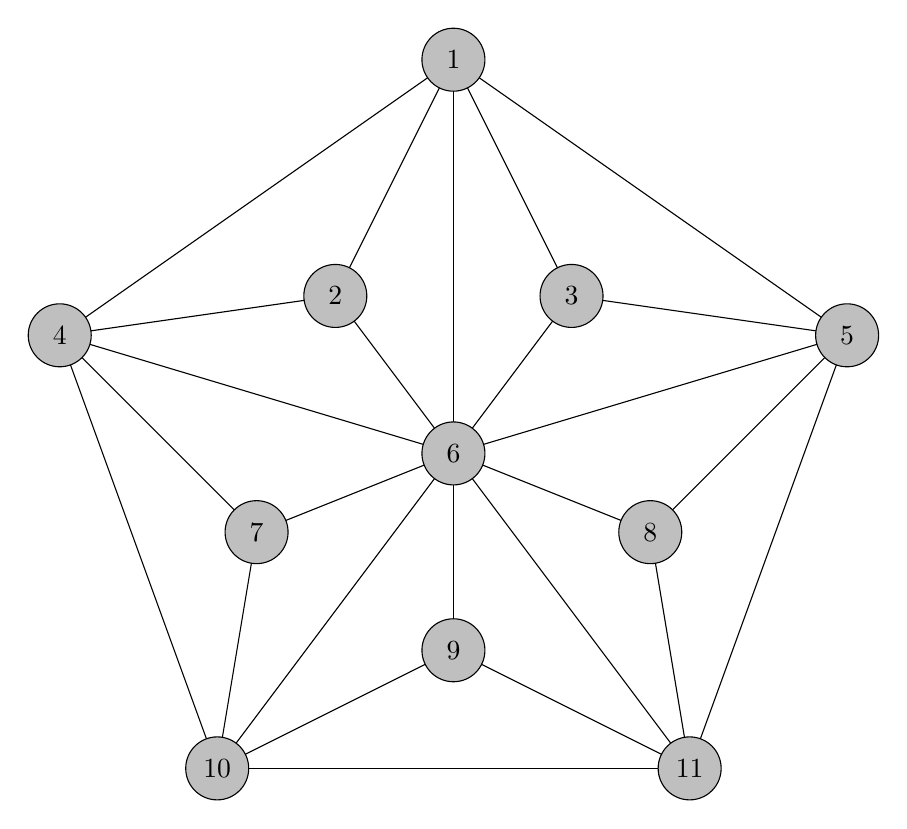
\begin{tikzpicture}
  \draw (7.5,12.5) -- (9,9.5); % 1 -- 3
  \draw (7.5,12.5) -- (12.5,9); % 1 -- 5
  \draw (6,9.5) -- (7.5,12.5); % 2 -- 1
  \draw (9,9.5) -- (12.5,9); % 3 -- 5
  \draw (2.5,9) -- (7.5,12.5); % 4 -- 1
  \draw (2.5,9) -- (6,9.5); % 4 -- 2
  \draw (12.5,9) -- (10,6.5); % 5 -- 8
  \draw (12.5,9) -- (10.5,3.5); % 5 -- 11
  \draw (7.5,7.5) -- (7.5,12.5); % 6 -- 1
  \draw (7.5,7.5) -- (6,9.5); % 6 -- 2
  \draw (7.5,7.5) -- (9,9.5); % 6 -- 3
  \draw (7.5,7.5) -- (2.5,9); % 6 -- 4
  \draw (7.5,7.5) -- (12.5,9); % 6 -- 5
  \draw (7.5,7.5) -- (5,6.5); % 6 -- 7
  \draw (7.5,7.5) -- (10,6.5); % 6 -- 8
  \draw (7.5,7.5) -- (7.5,5); % 6 -- 9
  \draw (7.5,7.5) -- (4.5,3.5); % 6 -- 10
  \draw (7.5,7.5) -- (10.5,3.5); % 6 -- 11
  \draw (5,6.5) -- (2.5,9); % 7 -- 4
  \draw (10,6.5) -- (10.5,3.5); % 8 -- 11
  \draw (7.5,5) -- (4.5,3.5); % 9 -- 10
  \draw (4.5,3.5) -- (2.5,9); % 10 -- 4
  \draw (4.5,3.5) -- (5,6.5); % 10 -- 7
  \draw (10.5,3.5) -- (7.5,5); % 11 -- 9
  \draw (10.5,3.5) -- (4.5,3.5); % 11 -- 10
  \filldraw[fill=lightgray] (7.5,12.5) circle (0.4) node{1};
  \filldraw[fill=lightgray] (6,9.5) circle (0.4) node{2};
  \filldraw[fill=lightgray] (9,9.5) circle (0.4) node{3};
  \filldraw[fill=lightgray] (2.5,9) circle (0.4) node{4};
  \filldraw[fill=lightgray] (12.5,9) circle (0.4) node{5};
  \filldraw[fill=lightgray] (7.5,7.5) circle (0.4) node{6};
  \filldraw[fill=lightgray] (5,6.5) circle (0.4) node{7};
  \filldraw[fill=lightgray] (10,6.5) circle (0.4) node{8};
  \filldraw[fill=lightgray] (7.5,5) circle (0.4) node{9};
  \filldraw[fill=lightgray] (4.5,3.5) circle (0.4) node{10};
  \filldraw[fill=lightgray] (10.5,3.5) circle (0.4) node{11};
\end{tikzpicture}

\end{center}
\end{document}
